\documentclass{article}
\usepackage[letterpaper, margin=1in]{geometry}
\usepackage{fancyhdr}
\usepackage[utf8]{inputenc}
\usepackage{amsmath}
\usepackage{circuitikz}
\usepackage{pgfplots}
\usepackage{bm}
\usepackage{amsfonts}
\usepackage{graphicx}
\usepackage{float}
\usepackage{subcaption}
\usepackage[dvipsnames]{xcolor}
\usepackage{array}
\usepackage[colorlinks=true, allcolors=blue]{hyperref}
\title{6. AC Steady-State Analysis \\  \large Introduction to Electric Circuits \\ Supplemental Instruction}
\author{Cooper McAllister}
\date{April 7 2026}
\begin{document}
\fancypagestyle{footerstyle} {
	\fancyhf{}
	\renewcommand{\headrulewidth}{0pt}
	\renewcommand{\footrulewidth}{0.4pt}
	\fancyfoot[L]{\textit{For personal study and students leading supplemental instruction, \\ with attribution given to the author. \\ Find more at coopermcallister.com}}
	\fancyfoot[R]{\thepage}
}
\pagestyle{footerstyle}
\maketitle
\thispagestyle{footerstyle}

\begin{center}
\textit{This document is not a substitute for a textbook or classroom instruction. It may contain errors and is intended to be used only to the extent that it is helpful to supplement students' learning experience.}
\end{center}

\section{Introduction}
We are now beginning our study of AC circuits! In AC, or Alternating Current, both voltage and current are sinusoidal functions of time, meaning they alternate back and forth between positive and negative values. Working with sinusoidal functions rather than simple numbers might appear difficult at first, but there are a number of mathematical tools and tricks we can use to simplify our analysis. Here I've attempted to condense these down into a minimal ''cheat sheet`` of what you need to know.

\section{The Sinusoidal Function}
Sinusoidal voltages and currents are written as
$$m(t) = M\cos(\omega t + \alpha)$$
where $M$ is the amplitude (sometimes called the peak amplitude), $\omega$ is the angular frequency (in rad/s), and $\alpha$ is the phase angle.
\\The angular frequency is related to the frequency by the equation
$$\omega = 2\pi f$$
Where $\omega$ is in rad/s and $f$ is in Hz.
The period $T$ of a sinusoidal function, in seconds, is
$$T = \frac{1}{f}$$
\\Note that the $\sin()$ function is not used (by convention). If a $\sin$ function was written in the standard form, it would be as $\cos(x - 90^\circ) = \sin(x)$.
\subsection*{Leading and Lagging Signals}
Let's say we have two sinusoidal signals of the same frequency, $v_1(t) = V_{1m}\cos(\omega t + \alpha_1)$ and $v_2(t) = V_{2m}\cos(\omega t + \alpha_2)$.
If $\alpha_1 > \alpha_2$, we say that $v_1$ \textbf{leads} $v_2$, and at the same time, $v_2$ \textbf{lags} $v_1$. Similarly, if $\alpha_2 > \alpha_1$, $v_2$ leads $v_1$, and $v_1$ lags $v_2$.


\section{Complex Number Review}
\subsection{Notation}
Recall that the imaginary unit is $i = \sqrt{-1}$. However, for circuits, we use $j$ instead of $i$ so as not to confuse it with current. A complex number can be written in \textbf{rectangular form} as
$$\bm{Z} = \mathcolor{red}{a} + \mathcolor{blue}{b}j$$
Where $ \mathcolor{red}{a = Re\{z\}}$ is the real part, and $\mathcolor{blue}{b = Im\{z\}}$ is the imaginary part. We can also draw a complex number as a vector in the complex plane:
\begin{figure}[H]
\centering
\begin{tikzpicture}
	\draw[<->] (-2,0)--(2,0) node[right]{$\mathbb{R}$};
	\draw[<->] (0,-2)--(0,2) node[above]{$\mathbb{I}$};
	\draw[line width=1pt,-stealth] (0, 0) -- (1.5, 1) node[anchor = north west] {$z$};
	\draw[red, line width = 0.7pt, |-|] (0, 0) -- (1.5, 0);
	\draw (0.75, -0.25) node[]{$\mathcolor{red}{a}$};
	\draw[blue, line width = 0.7pt, |-|] (0, 0) -- (0, 1);
	\draw (-0.25, 0.5) node[]{$\mathcolor{blue}{b}$};
\end{tikzpicture}
\end{figure}
Another way to write complex numbers is \textbf{polar form}:
$$\bm{Z} = Z_m \angle \theta$$
Where $Z_m$ is the magnitude and $\theta$ is the angle. The $\angle$ symbol can be pronounced "angle". 
An equivalent notation for polar form is
$$\bm{Z} = Z_m e^{j\theta}$$
We can convert between polar and rectangular forms using
$$Z_m = \sqrt{a^2 + b^2}, \qquad \tan(\theta) = \frac{b}{a}$$
Many scientific and graphing calculators have built-in functions that can do these conversions.
\subsection{Complex Multiplication and Division}
Let's say we have two complex numbers, $\bm{X} = X_m \angle \alpha$ and $\bm{Y} = Y_m \angle \beta$. We can write their product as
$$\bm{X}\bm{Y} = X_me^{j\alpha}\cdot Y_me^{j\beta} = X_m\cdot Y_m e^{j\alpha + j\beta} = X_m \cdot Y_m e^{j(\alpha + \beta)} = X_m\cdot Y_m \angle (\alpha + \beta)$$
We can also divide complex numbers:
$$\frac{\bm{X}}{\bm{Y}} = \frac{X_me^{j\alpha}}{Y_me^{j\beta}} = \frac{X_m}{Y_m}e^{j\alpha - j\beta} = \frac{X_m}{Y_m} \angle (\alpha - \beta)$$
\subsection{A Note on the Complex Unit}
Note that, using polar form, $j = 1\angle 90^\circ$. Also, it can be shown using the division formula above that $\frac{1}{j} = -j$.

\section{The Phasor (yes, they're really called that, it's awesome)}
Using math, it is possible to write a sinusoidal function in the \textit{time domain} as a \textbf{phasor} in the \textit{frequency domain}:
$$m(t) = M\cos(\omega t + \alpha) \Rightarrow \bm{M}(t) = Me^{j(\omega t + \alpha)}$$
$\bm{M}(t)$ is a vector in the complex plane that rotates counterclockwise over time, with magnitude $M$ and angle $(\omega t + \alpha)$. Below is a graphical representation of a sinusoidal function and its phasor representation. We usually draw phasors at time $t=0$, so the phase angle $\alpha$ is the angle between the phasor and the positive real axis.

\begin{figure}[H]
\centering
\begin{subfigure}[b]{0.4\textwidth}
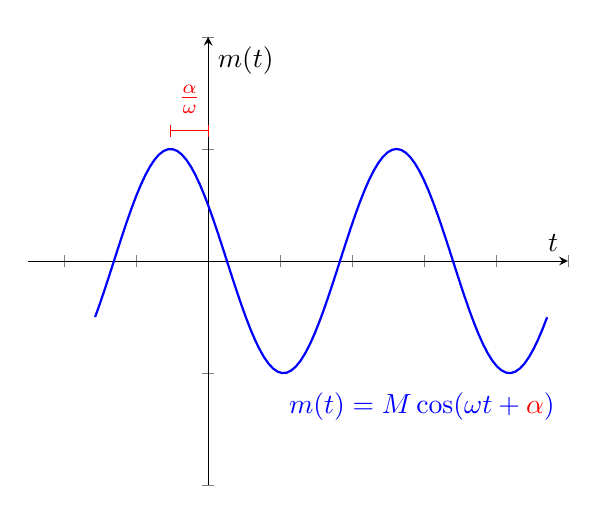
\begin{tikzpicture}
\begin{axis}[
	        	axis lines = middle,
	        	xlabel = $t$,
	        	ylabel = {$m(t)$},
	        	ymin=-2, ymax=2,
	        	xmin=-5, xmax=10,
	        	xtick={},
	        	xticklabels={},
		yticklabels={}
    	]
    	% Plot sin(x)
    	\addplot [
	        domain=-pi:3*pi,
	        samples=100,
	        color=blue,
	        thick
    	] {cos(deg(x) + 60)};
\end{axis}
\draw (5, 1) node[]{$\mathcolor{blue}{m(t) = M\cos(\omega t + \mathcolor{red}{\alpha})}$};
\draw[color=red, |-|] (2.3, 4.5) -- (1.8, 4.5);
\draw (2.05, 4.9) node[]{$\mathcolor{red}{\frac{\alpha}{\omega}}$};
\end{tikzpicture}
\caption*{Time Domain (sinusoidal function)}
\end{subfigure}
\hfill
\begin{subfigure}[b]{0.4\textwidth}
\centering
\begin{tikzpicture}
	\draw[<->] (-3,0)--(3,0) node[right]{$\mathbb{R}$};
	\draw[<->] (0,-3)--(0,3) node[above]{$\mathbb{I}$};
	\draw[line width=1pt,blue,-stealth] (0, 0) -- (1, 1.732) node[anchor = north west] {$\bm{M} = Me^{j(\omega t + \mathcolor{red}{\alpha})}$};
	\draw[red] (0.707,0) arc (0:60:0.707);
	\draw (0.9, 0.4) node[]{$\mathcolor{red}{\alpha}$};
	\draw[->] (0.44,0.9) arc (45:120:1.1);
	\draw (-1.2, 1) node[]{$\omega t$};
\end{tikzpicture}
\caption*{Frequency Domain (phasor)}
\end{subfigure}
\end{figure}


\subsection*{Phasor Notation}
In this class we only work with circuits in which every time-varying value is a sinusoid of the same frequency. Therefore, the $\omega t$ term is present in every phasor, so we usually abbreviate by omitting it and writing a phasor as simply
$$m(t) = M\cos(\omega t + \alpha) \Rightarrow \bm{M} = Me^{j\alpha}$$
Or, using abbreviated polar form notation:
$$\bm{M} = M\angle\alpha$$
Phasors can also be written in rectangular form:
$$\bm{M} = a + bj, \quad a=M\cos(\alpha), \quad b=M\sin(\alpha)$$
Below is a visual representation of some different phasors using the abbreviated polar form:
\begin{figure}[H]
\centering
\begin{subfigure}[b]{0.4\textwidth}
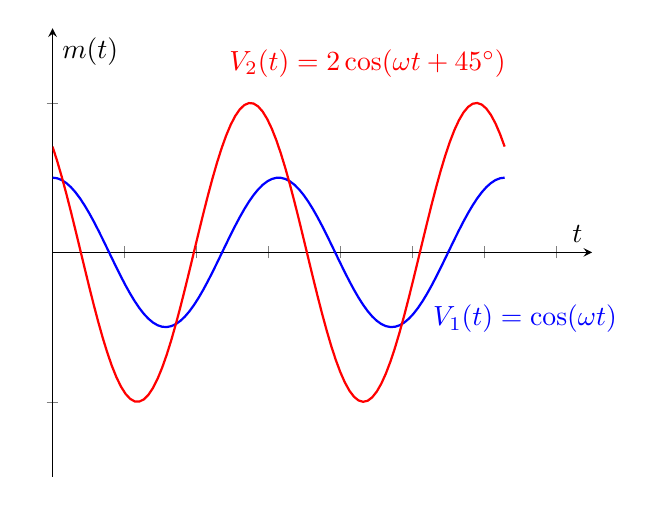
\begin{tikzpicture}
\begin{axis}[
	        	axis lines = middle,
	        	xlabel = $t$,
	        	ylabel = {$m(t)$},
	        	ymin=-3, ymax=3,
	        	xmin=0, xmax=15,
	        	xtick={},
	        	xticklabels={},
		yticklabels={}
    	]
    	% Plot sin(x)
    	\addplot [
	        domain=0:4*pi,
	        samples=100,
	        color=blue,
	        thick
    	] {cos(deg(x))};
    	\addplot [
	        domain=0:4*pi,
	        samples=100,
	        color=red,
	        thick
    	] {2*cos(deg(x) +45)};
\end{axis}
\draw (6, 2) node[]{$\mathcolor{blue}{V_1(t) = \cos(\omega t)}$};
\draw (4, 5.25) node[]{$\mathcolor{red}{V_2(t) =2\cos(\omega t + 45^{\circ})}$};
\end{tikzpicture}
\caption*{Time Domain (sinusoidal function)}
\end{subfigure}
\hfill
\begin{subfigure}[b]{0.4\textwidth}
\centering
\begin{tikzpicture}
	\draw[<->] (-3,0)--(3,0) node[right]{$\mathbb{R}$};
	\draw[<->] (0,-3)--(0,3) node[above]{$\mathbb{I}$};
	\draw[line width=1pt,blue,-stealth] (0, 0) -- (1, 0) node[anchor = north west] {$\bm{V_1} = 1\angle 0^\circ$};
	\draw[line width=1pt,red,-stealth] (0, 0) -- (1.41, 1.41) node[anchor = west] {$\bm{V_2} = 2\angle 45^\circ$};
	\draw[->] (0.5,0.125) arc (10:120:0.5);
	\draw[->] (0.707,0.85) arc (48:120:1.05);
	\draw (-0.75, 0.65) node[]{$\omega t$};
\end{tikzpicture}
\caption*{Frequency Domain (phasor)}
\end{subfigure}
\end{figure}
\subsection*{Handwriting Phasors}
In typed documents such as this, phasors are written using a bold font: $\bm{V}$. However, in handwriting, a dot is written above the symbol to specify that is is a phasor: $\dot{V}$.

\section{Impedance}
All of the circuit analysis we've done up to this point works the same way in the frequency domain, but every current and voltage is a complex number (a phasor). The equivalent of resistance when working with phasors is impedance ($\bm{Z}$), which is a complex number but not a phasor (it doesn't rotate over time). For any impedance $\bm{Z}$, Ohm's Law is true in the frequency domain:
$$\bm{V} = \bm{I}\cdot\bm{Z}$$
The unit of impedance is Ohms ($\Omega$).
The impedance of various components can be found as follows: \\ \\ 

\begin{center}
\begin{tabular}{ | m{5em} | m{9em} | m{5em} | } 
 \hline
 Resistor & \begin{circuitikz}[american, cute inductors] \draw
(0, 0) to[R=$R$] (3, 0)
;
\end{circuitikz} & $\bm{Z_R} = R$ \\ 
\hline
 Inductor & \begin{circuitikz}[american, cute inductors] \draw
(0, 0) to[inductor, l=$L$] (3, 0)
;
\end{circuitikz} & $\bm{Z_L} = j\omega L$ \\ 
\hline
 Capacitor & \begin{circuitikz}[american, cute inductors] \draw
(0, 0) to[capacitor, l=$C$] (3, 0)
;
\end{circuitikz} & $\bm{Z_C} = \frac{1}{j\omega C}$ \\ 
 \hline
\end{tabular}
\end{center}

In rectangular form, impedance is written as 
$$\bm{Z} = R + Xj$$
where $R$ is resistance, and $X$ is called \textbf{reactance}, and both have units of Ohms ($\Omega$). Note that reactance is a real number (it does not include $j$). For an inductor, $X = \omega L$, and for a capacitor, $X = \frac{-1}{\omega C}$. Note that resistors have zero reactance, inductors have positive reactance, and capacitors have negative reactance. However, sometimes capacitor reactance is written as a positive number, $X_c = \frac{1}{\omega C}$; in this case the negative sign is implied.

\subsection*{Admittance and Susceptance}
The reciprocal of impedance is admittance, $\bm{Y}$:
$$\bm{Y} = \frac{1}{\bm{Z}}$$
In rectangular form,
$$\bm{Y} = G + jB$$
Where $G$ is conductance, and $B$ is called \textbf{Susceptance}, and both have unites of Siemens (s).

\subsection*{Current and Voltage in a Capacitor}
In a capacitor, current leads voltage by $90^\circ$:
\begin{figure}[H]
\centering
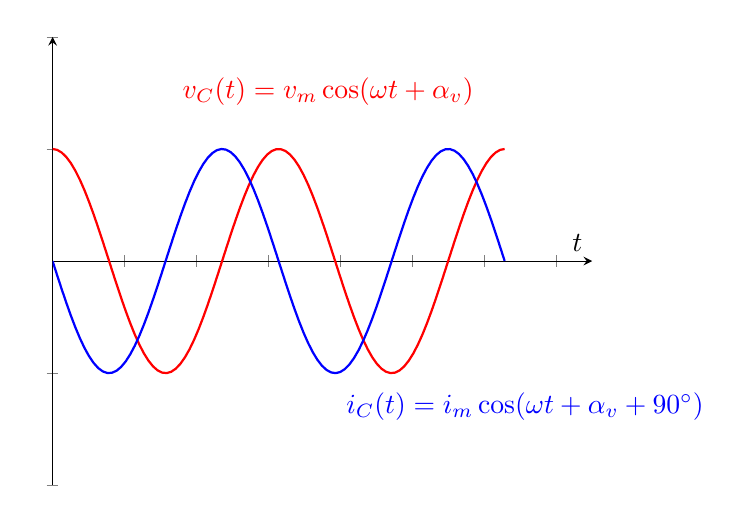
\begin{tikzpicture}
\begin{axis}[
	        	axis lines = middle,
	        	xlabel = $t$,
	        	ymin=-2, ymax=2,
	        	xmin=0, xmax=15,
	        	xtick={},
	        	xticklabels={},
		yticklabels={}
    	]
    	% Plot sin(x)
    	\addplot [
	        domain=0:4*pi,
	        samples=100,
	        color=red,
	        thick
    	] {cos(deg(x))};
    	\addplot [
	        domain=0:4*pi,
	        samples=100,
	        color=blue,
	        thick
    	] {*cos(deg(x) + 90)};
\end{axis}
\draw (3.5, 5) node[]{$\mathcolor{red}{v_C(t) = v_m\cos(\omega t + \alpha_v)}$};
\draw (6, 1) node[]{$\mathcolor{blue}{i_C(t) = i_m\cos(\omega t + \alpha_v + 90^\circ)}$};
\end{tikzpicture}
\end{figure}
\subsection*{Current and Voltage in an Inductor}
In an inductor, current lags voltage by $90^\circ$:
\begin{figure}[H]
\centering
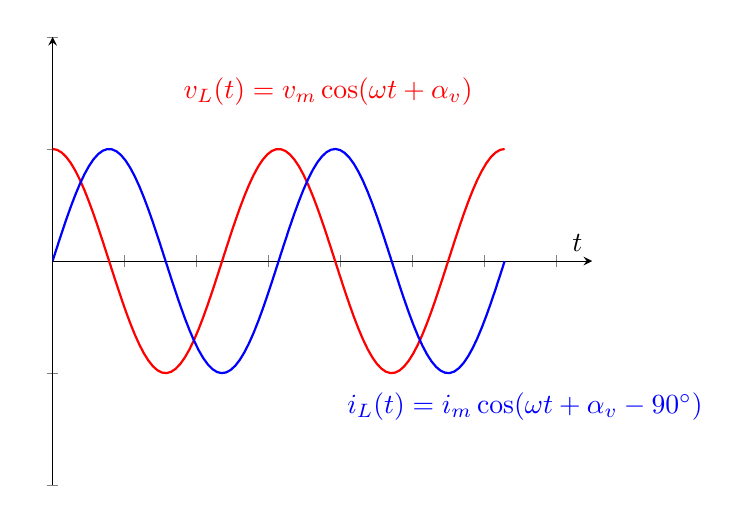
\begin{tikzpicture}
\begin{axis}[
	        	axis lines = middle,
	        	xlabel = $t$,
	        	ymin=-2, ymax=2,
	        	xmin=0, xmax=15,
	        	xtick={},
	        	xticklabels={},
		yticklabels={}
    	]
    	% Plot sin(x)
    	\addplot [
	        domain=0:4*pi,
	        samples=100,
	        color=red,
	        thick
    	] {cos(deg(x))};
    	\addplot [
	        domain=0:4*pi,
	        samples=100,
	        color=blue,
	        thick
    	] {cos(deg(x) - 90)};
\end{axis}
\draw (3.5, 5) node[]{$\mathcolor{red}{v_L(t) = v_m\cos(\omega t + \alpha_v)}$};
\draw (6, 1) node[]{$\mathcolor{blue}{i_L(t) = i_m\cos(\omega t + \alpha_v - 90^\circ)}$};
\end{tikzpicture}
\end{figure}
The above statements can be proven using either phasors and impedance or time domain analysis. 

\section{Appendix: Why Complex Numbers Work for Circuit Analysis}
\subsection*{Laplace Domain Analysis}
Remember that for an inductor, $v_L(t) = L\frac{di_L(t)}{dt}$, and for a capacitor, $i_C(t) = C\frac{dv_C(t)}{dt}$, which means $v_C(t) = \frac{1}{C}\int i_C(t)$ (ignoring initial conditions). When we take the Laplace transform, we treat differentiation as multiplication by $s$, and integration as division by $s$. Therefore, taking the Laplace transform, we get 
$$V_L(s) = LsI_L(s) \qquad \textrm{and} \qquad V_C(s) = \frac{I_C(s)}{Cs}$$ 
If we substitute $s = j\omega$\footnote{The reasoning behind this substitution is not something I am able to explain. I would recommend \href{https://www.youtube.com/watch?v=j0wJBEZdwLs}{3Blue1Brown's youtube series on the topic} for those who want to learn more.}, we get
$$V_L(s) = j\omega L I_L(s) \qquad \textrm{and} \qquad V_C(s) = \frac{I_C(s)}{j\omega C}$$
We can now substitute the impedances $Z_L = j\omega L$ and $Z_C = \frac{1}{j\omega C}$:
$$V_L(s) = Z_L I_L(s) \qquad \textrm{and} \qquad V_C(s) = Z_C I_C(s)$$
And we have arrived at Ohm's Law in the frequency domain.
\subsection*{Treating multiplication by $j\omega$ as differentiation}
Another way of looking at this is as follows. If we have an inductor with some current $i(t) = I_m\cos(\omega t + \alpha)$, the voltage will be
$$v(t) = L\cdot\frac{di(t)}{dt} = L\cdot-I_m\omega\sin(\omega t + alpha)$$
We can use the trig identity $-\sin(x) = \cos(x + 90^\circ)$ to simplify:
$$v(t) = L\cdot I_m\omega\cos(\omega t + \alpha + 90^\circ)$$
We can write this as a phasor:
$$\bm{V} = LI_m\omega \angle (\alpha + 90^\circ)$$
Using Ohm's Law, we can equate this voltage to the current times the impedance:
$$\bm{V} = LI_m\omega \angle (\alpha + 90^\circ) = \bm{I}\bm{Z_L}$$
Let's write the impedance and current in polar form with an impedance magnitude $Z_m$ and phase angle $\theta$.
$$\bm{V} = LI_m\omega \angle (\alpha + 90^\circ) = I_m \angle \alpha \cdot Z_L \angle \theta_L = I_mZ_L \angle (\alpha + \theta_L)$$
Equating the magnitude and angle:
$$LI_m\omega = I_mZ_L \Rightarrow Z_L = L\omega$$
$$\alpha + 90^\circ = \alpha + \theta_L \Rightarrow \theta_L = 90^\circ$$
Writing $\bm{Z_L}$ in rectangular form,
$$\bm{Z_L}= j\omega L$$
We can find the impedance of a capacitor in a similar manner.



\newpage
\section*{References}
\begin{itemize}
\item M. Iordache. Class Lectures, Topic: ``Electric circuits.'' EEGR 2053, School of Engineering and Engineering Technology, LeTourneau University, 2025.
\item M. Iordache. 2024. EEGR 2053 Electric circuits [PowerPoint slides]. Available: \\ https://mviordache.name/EEGR2053/index.html
\item T. L. Floyd and D. M. Buchla, Principles of Electric Circuits: Conventional Current, 10th ed. Hoboken, NJ: Pearson Education, 2020.
\item O. Ortiz. 2025. ENGR 2053 Intro to electric circuits [PowerPoint slides].
\end{itemize}

	
\end{document}